\documentclass[t]{beamer}
\usetheme{CambridgeUS}

\usepackage{minted}
\usepackage{colortbl}
\usepackage{hyperref}

\title{LDA and Information Retrieval}
\author{Jaimie Murdock}
\institute[IU COGS]{
    IU Cognitive Science Program\\
    810 Eigenmann Hall\\
    \texttt{jammurdo@indiana.edu}
    }
\date{November 12, 2014}

\begin{document}
% Title Page
\frame{\titlepage}
\frame{\tableofcontents}

\section{Introduction}
\subsection{VSM}
\begin{frame}
\frametitle{Vector Space Model}
Comparison of \textbf{word} space \\
Document is a vector \\
Query is also a vector

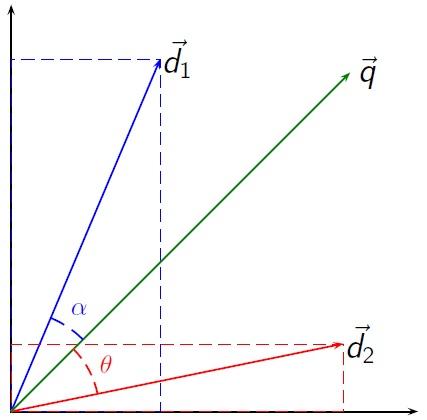
\includegraphics[width=0.4\textwidth]{img/vsm.jpg}

\cite{salton1975}
\end{frame}

\subsection{LSA}
\begin{frame}
\frametitle{Latent Semantic Analysis}
Comparison of \textbf{document} space \\
Latent variables are dimensions \\
Groups together related terms

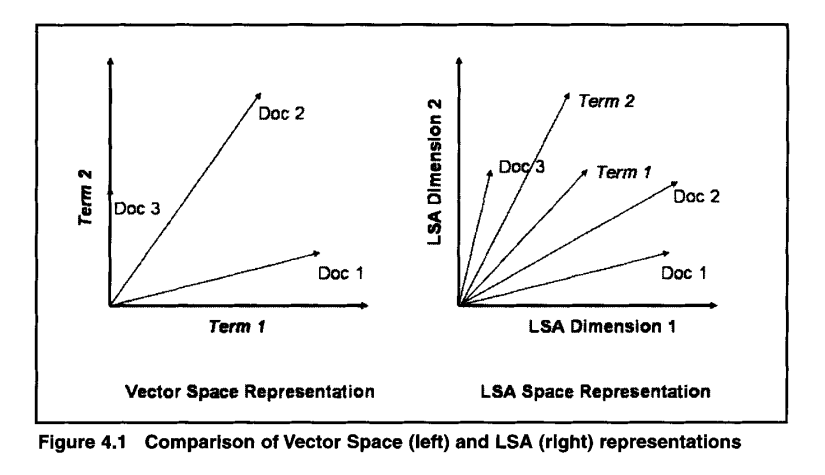
\includegraphics[width=0.8\textwidth]{img/vsm-vs-lsa.png}

\cite{deerwester1990,dumais2005}
\end{frame}

\begin{frame}
\frametitle{Latent Semantic Analysis}
Uses \textbf{singular value decomposition} (SVD) \\
to determine \textbf{latent} variables

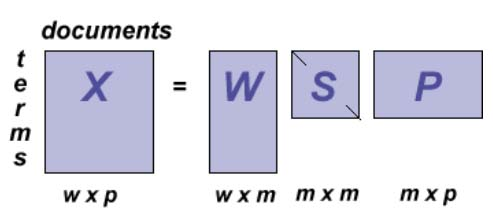
\includegraphics[width=0.8\textwidth]{img/lsa.jpg}

\cite{deerwester1990,dumais2005}
\end{frame}

\subsection{LDA}
\begin{frame}
\frametitle{Latent Dirichlet Allocation}
Generative model of \textbf{topic} space

%\begin{figure}
%\def\svgwidth{0.7\textwidth}
%\input{img/lda.pdfx}
%\end{figure}
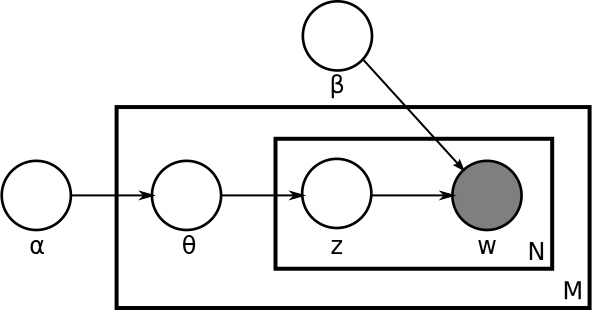
\includegraphics[width=0.5\textwidth]{lda.pdf}

\begin{itemize}
\item $K$ -- the number of topics
\item $M$ -- the number of documents
\item $N$ -- number of words in document
\item $V$ -- the number of unique words across all documents
\item $\alpha$ -- prior distribution of per-document topic distributions
\item $\beta$ -- prior distribution of per-topic word distributions
\end{itemize}

\cite{Blei2003}
\end{frame}

\begin{frame}
\frametitle{Latent Dirichlet Allocation}

%\begin{figure}
%\def\svgwidth{0.7\textwidth}
%\input{img/lda.pdfx}
%\end{figure}
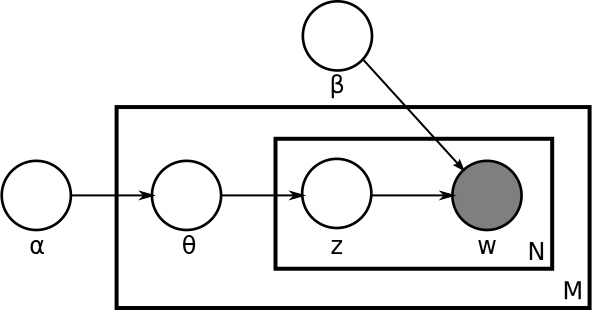
\includegraphics[width=0.5\textwidth]{lda.pdf}

\begin{itemize}
\item $\theta_i$ -- the topic distribution for document $i$ ($MxK$)
\item $\phi_k$ -- the word distribution for topic $k$ ($KxV$)
\item $z_{ij}$ -- the topic assignment for the $j$th word in document $i$
\item $w_{ij}$ -- the specific word
\end{itemize}

\cite{Blei2003}
\end{frame}

\begin{frame}
\frametitle{Latent Dirichlet Allocation}

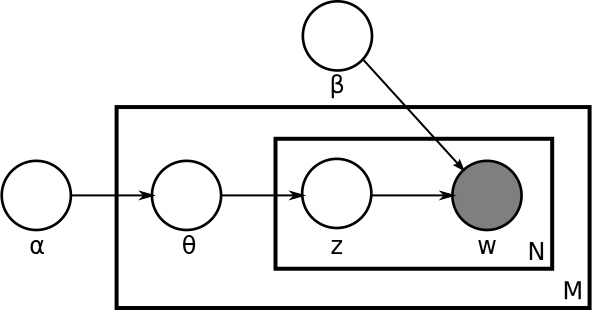
\includegraphics[width=0.5\textwidth]{lda.pdf}
\bigskip

\textbf{Generative Model}
\begin{enumerate}
\item Choose $\theta_i \sim Dir(\alpha)$
\pause
\item Choose $\phi_k \sim Dir(\beta)$
\pause
\item For each word $i, j$:
    \begin{itemize}
    \item Choose a topic $z_{ij} \sim Multinomial(\theta_i)$
    \item Choose a word $w_{ij} \sim Multinomial(\phi_k)$
    \end{itemize}
\end{enumerate}

\cite{Blei2003}
\end{frame}

\section{Visualizations}
\subsection{Termite}
\begin{frame}
\frametitle{Termite}
\textbf{Type:} word-topic, topic-topic

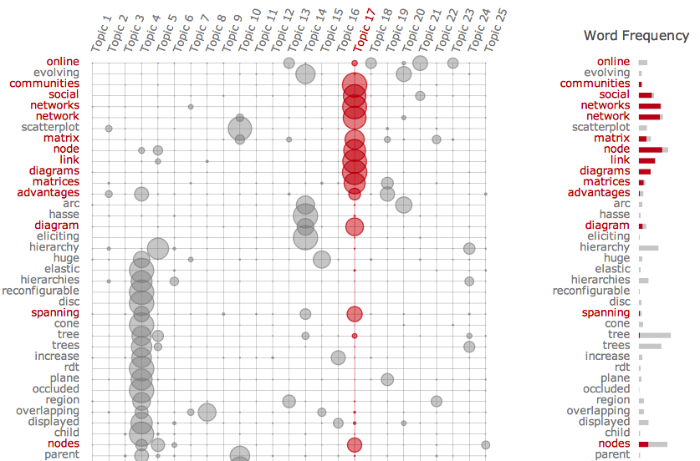
\includegraphics[width=0.75\textwidth]{img/termite.png}

\url{http://vis.stanford.edu/papers/termite}

\cite{Chuang2012}
\end{frame}

\subsection{LDAvis}
\begin{frame}
\frametitle{LDAvis}
\textbf{Type:} word-word, word-topic, topic-topic

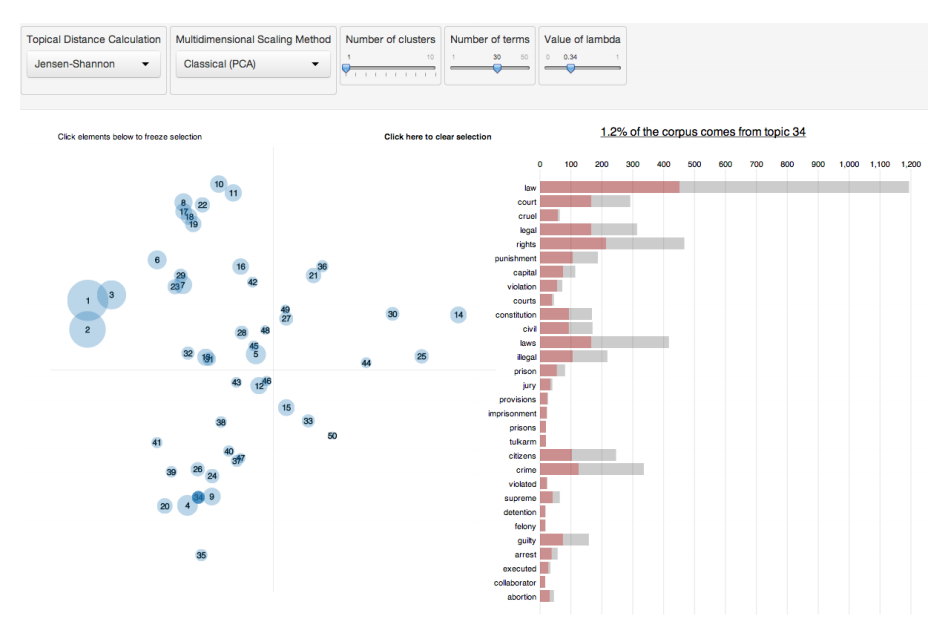
\includegraphics[width=0.75\textwidth]{img/ldavis.png}


\url{http://www2.research.att.com/~kshirley/lda/}

\cite{Sievert2014}
\end{frame}

\subsection{Topic Explorer}
\begin{frame}
\frametitle{Topic Explorer}
\textbf{Type:} document-document, document-topic, topic-topic

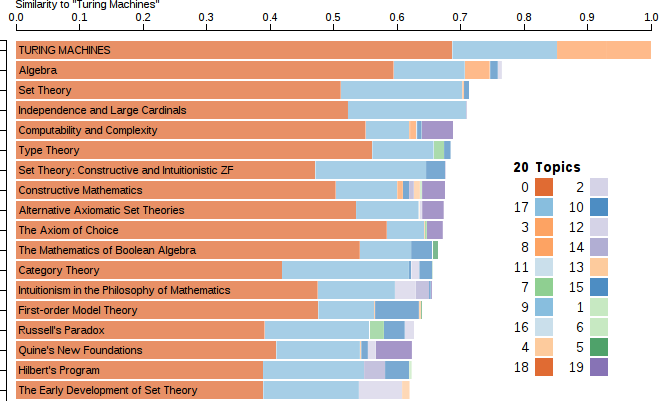
\includegraphics[width=0.75\textwidth]{img/topex20.png}
\url{http://inphodata.cogs.indiana.edu/}

\cite{aaai2015}
\end{frame}

\begin{frame}
\frametitle{Topic Explorer}
\textbf{Type:} document-document, document-topic, topic-topic

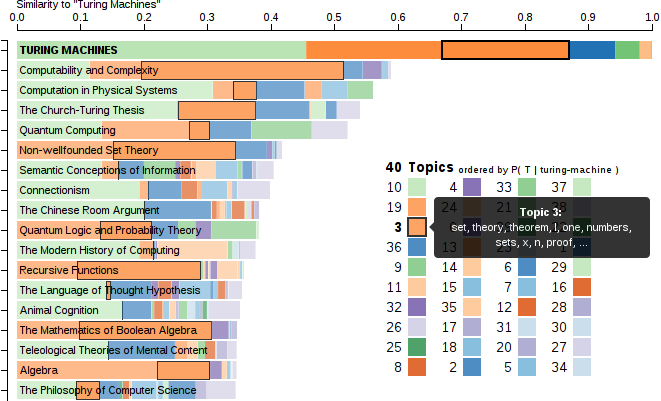
\includegraphics[width=0.75\textwidth]{img/topex40.png}

\url{http://inphodata.cogs.indiana.edu/}

\cite{aaai2015}
\end{frame}

\begin{frame}
\frametitle{Topic Explorer}
\textbf{Type:} document-document, document-topic, topic-topic

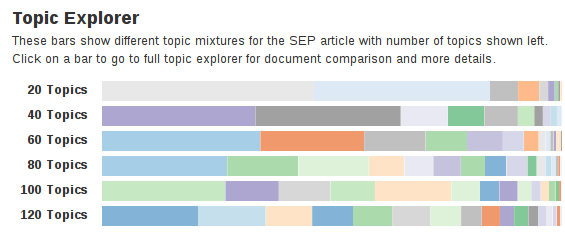
\includegraphics[width=0.75\textwidth]{img/topex-comparison.png}

\url{http://inphodata.cogs.indiana.edu/}

\cite{aaai2015}
\end{frame}

\section{Project}
\begin{frame}
\frametitle{Project Proposal (Part 1)}
Expand topic explorer similarity dimensions to include \textbf{words}.
\begin{itemize}
\item document-document
\item topic-document
\item topic-topic
\item \textbf{word-document}
\item \textbf{word-topic}
\end{itemize}
\end{frame}

\begin{frame}
\frametitle{Project Prpoposal (Part 2)}
Compare results of topic-model driven similarity\\
to Lucene similarity with parameterized search.

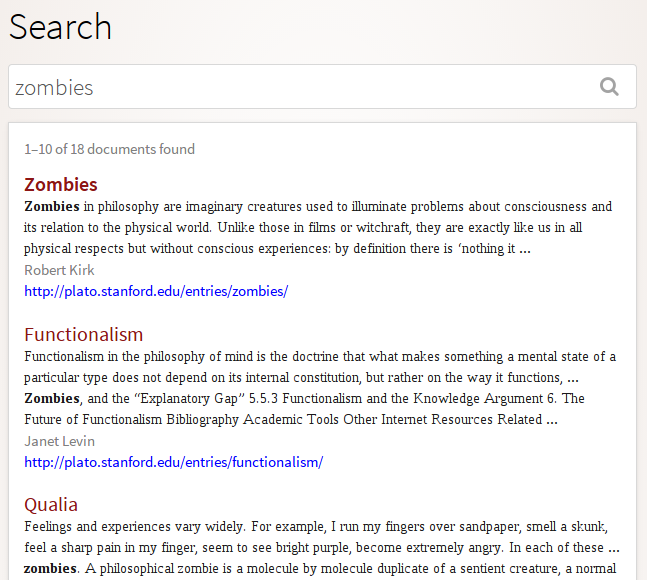
\includegraphics[width=0.75\textwidth]{img/zombie-lucene.png}

\url{http://plato.stanford.edu/search/searcher.py?query=zombies}
\end{frame}

\begin{frame}
\frametitle{Project Prpoposal (Part 2)}
Compare results of topic-model driven similarity\\
to Lucene similarity with search queries.

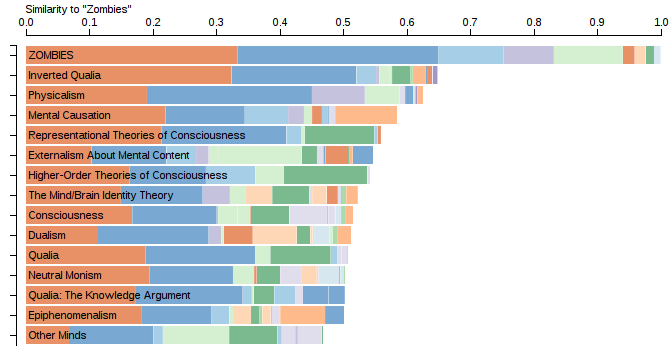
\includegraphics[width=0.75\textwidth]{img/topex-zombies.png}

\url{http://inphodata.cogs.indiana.edu:16040/?doc=zombies}
\end{frame}

\section{References}
\begin{frame}
\tiny
\bibliographystyle{apalike}
\bibliography{refs}
\end{frame}

\frame{\titlepage}

\end{document}
